% +------------------------------------------------------------------------+
% | Reference manual page: Subdivision_surfaces_3.tex
% +------------------------------------------------------------------------+
% | 03/01/2005   Le-Jeng Andy Shiue
% | Package: Subdivision_surface_3
% | 
\RCSdef{\RCSSubdivisionRev}{$Revision$}
\RCSdefDate{\RCSSubdivisionDate}{$Date$}
% +------------------------------------------------------------------------+

\ccRefPageBegin

%%RefPage: end of header, begin of main body
% +------------------------------------------------------------------------+


\begin{ccRefClass}{PQQ_stencil_3<Poly>}

\ccDefinition

A stencil maps an input control submesh to a node on the refined 
mesh. \ccClassTemplateName\ defines the policy interface of 
stencils of the PQQ refinement. Served as the programming guideline,
\ccClassTemplateName\ does not realize any specific geometry mask.
Since stencil interfaces of the PTQ and the $\sqrt{3}$ refinements are
in nature subsets of the PQQ refinement, \ccClassTemplateName\ can 
be used to derive geometry masks for the PTQ and the $\sqrt{3}$ refinement.

%% \begin{ccTexOnly}
%%     \vspace{-7mm}
%%     \begin{center}
%%       \parbox{0.4\textwidth}{%
%%         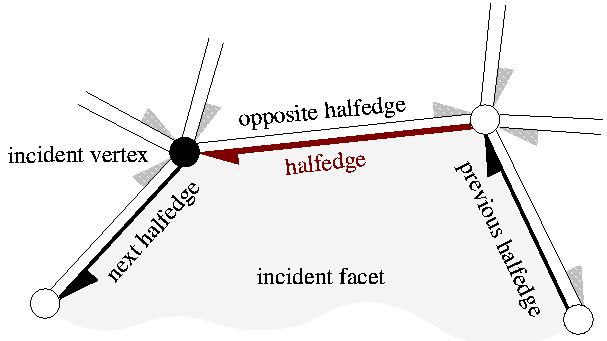
\includegraphics[width=0.4\textwidth]{Polyhedron_ref/fig/halfedge}%
%%       }
%%     \end{center}
%%     \vspace{-5mm}
%% \end{ccTexOnly}

%% \begin{ccHtmlOnly}
%%     <CENTER>
%%     <A HREF="fig/halfedge.gif">
%%         <img src="fig/halfedge_small.gif" alt="Halfedge Diagram"></A><P>
%%     </CENTER>
%% \end{ccHtmlOnly}

\ccInclude{CGAL/Subdivision_surfaces_masks_3.h}

\ccParameters

The full template declaration of \ccClassTemplateName\ states one
template parameter:

\begin{tabbing}
\ccc{template <} \=\ccc{class Polyhedron_3>} \ccc{class PQQ_stencil_3;}
\end{tabbing}
   
The only parameter requires a model of 
the \ccc{Polyhedron_3} concept as argument. \ccc{Point_3} 
is required to be type-defined in \ccc{Polyhedron_3}.

%% \ccTypes

%% \ccNestedType{Traits}{traits class selected for \ccc{PolyhedronTraits_3}.}
%% \ccGlue
%% \ccNestedType{Items}{items class selected for \ccc{PolyhedronItems_3}.}
%% \ccGlue



%% % +-----------------------------------+
%% \begin{ccAdvanced}
%% \ccHeading{Types for Tagging Optional Features}

%% \ccNestedType{Supports_facet_plane}{\ccc{Facet::plane()}.}
%% \ccGlue
%% \ccNestedType{Supports_removal}{supports removal of individual elements.}

%% \end{ccAdvanced}

\ccCreation
\ccCreationVariable{P}

%\ccClassTemplateName\ is a functor of the three geometry stencils for
%subdivision surfaces based on the PQQ refinement. 
Default constructors are generated by the compiler.


% +-----------------------------------+
\ccHeading{Stencil Policies}
%\ccThree{void}{facet_node(Facet_handle f, Point& pt);}{}
\ccThree{void}{P.nn}{}
\ccThreeToTwo

\ccMethod{
void facet_node(Facet_handle f, Point& pt);
}{
define the access interface of the facet-node stencil.
\ccc{pt} is semantically required to be smoothed by averaging 
points of the neighborhood of \ccc{f}.
Override this function to support geometry masks for subdivisions 
based on the PQQ and the $\sqrt{3}$ refinement.
} 

\ccMethod{
void edge_node(Edge_handle e, Point& pt);
}{
define the access interface of the edge-node stencil. 
\ccc{pt} is semantically required to be smoothed by 
averaging points of the neighborhood of \ccc{e}.
Override this function to support geometry masks for subdivisions 
based on the PQQ and the PTQ refinement.
} 

\ccMethod{
void vertex_node(Vertex_handle v, Point& pt);
}{
define the access interface of the vertex-node stencil.
\ccc{pt} is semantically required to be smoothed by averaging 
points of the neighborhood of \ccc{v}.
Override this function to support geometry masks for subdivisions 
based on the PQQ, the PTQ and the $\sqrt{3}$ refinement.
} 


%% \begin{ccTexOnly}
%%     \begin{center}
%%       \parbox{0.636\textwidth}{%
%%           \includegraphics[width=0.636\textwidth]%
%%               {Polyhedron_ref/fig/euler_loop}%
%%       }
%%     \end{center}
%% \end{ccTexOnly}
%% \begin{ccHtmlOnly}
%%     <CENTER>
%%     <img src="fig/euler_loop.gif" alt="Euler Operator: Loop"><P>
%%     </CENTER>
%% \end{ccHtmlOnly}


\ccSeeAlso

\ccRefIdfierPage{CGAL::Subdivision_surfaces_3<Poly>}\\
\ccRefIdfierPage{CGAL::DQQ_stencil_3<Poly>}\\
\ccRefIdfierPage{CGAL::Linear_mask_3<Poly>}\\
\ccRefIdfierPage{CGAL::CatmullClark_mask_3<Poly>}\\
\ccRefIdfierPage{CGAL::Loop_mask_3<Poly>}\\
\ccRefIdfierPage{CGAL::Sqrt3_mask_3<Poly>}\\

%\ccExample
%This example program instantiates a polyhedron using the default
%traits class and creates a tetrahedron.
%\ccIncludeExampleCode{Polyhedron/polyhedron_prog_simple.C}

\end{ccRefClass}

% +------------------------------------------------------------------------+
%%RefPage: end of main body, begin of footer
\ccRefPageEnd
% EOF



% +------------------------------------------------------------------------+
% +------------------------------------------------------------------------+
\ccRefPageBegin

%%RefPage: end of header, begin of main body
% +------------------------------------------------------------------------+

\begin{ccRefClass}{DQQ_stencil_3<Poly>}

\ccDefinition

A stencil maps an input control submesh to a node on the refined 
mesh. \ccClassTemplateName\ defines the policy interface of 
stencils of the DQQ refinement. Served as the programming guideline,
\ccClassTemplateName\ does not realize any specific geometry mask.

\ccInclude{CGAL/Subdivision_surfaces_masks_3.h}

\ccParameters

The full template declaration of \ccClassTemplateName\ states one
template parameter:

\begin{tabbing}
\ccc{template <} \=\ccc{class Polyhedron_3>} \ccc{class DQQ_stencil_3;}
\end{tabbing}
   
The only parameter requires a model of 
the \ccc{Polyhedron_3} concept as argument. \ccc{Point_3} 
is required to be type-defined in \ccc{Polyhedron_3}.

\ccCreation
\ccCreationVariable{P}

Default constructors are generated by the compiler.


% +-----------------------------------+
\ccHeading{Stencil Policies}
%\ccThree{void}{corner_node(Halfedge_handle he, Point& pt);}{}
\ccThree{void}{P.nn}{}
\ccThreeToTwo

\ccMethod{
void corner_node(Halfedge_handle he, Point& pt);
}{
define the access interface of the corner-node stencil 
of the DQQ refinement. 
\ccc{pt} is semantically required to be smoothed by averaging 
points on the facet of \ccc{he}. \ccc{he} always points to the vertex 
that usually has the dominate mask weight.
}

\ccSeeAlso

\ccRefIdfierPage{CGAL::Subdivision_surfaces_3<Poly>}\\
\ccRefIdfierPage{CGAL::PQQ_stencil_3<Poly>}\\
\ccRefIdfierPage{CGAL::DooSabin_mask_3<Poly>}\\

\end{ccRefClass}

% +------------------------------------------------------------------------+
%%RefPage: end of main body, begin of footer
\ccRefPageEnd
% EOF
% +------------------------------------------------------------------------+



% +------------------------------------------------------------------------+
% +------------------------------------------------------------------------+
\begin{ccRefClass}{Linear_mask_3<Poly>}

\ccDefinition

\ccClassTemplateName , inherited the policy interface from
\ccc{PQQ_stencil_3}, realizes the geometry masks as bi-linear 
averaging of nodes collected from the stencils.

\ccInclude{CGAL/Subdivision_surfaces_masks_3.h}

\ccParameters

The full template declaration of \ccClassTemplateName\ states one
template parameter:

\begin{tabbing}
\ccc{template <} \=\ccc{class Polyhedron_3>} \ccc{class Linear_mask_3;}
\end{tabbing}
   
The only parameter requires a model of 
the \ccc{Polyhedron_3} concept as argument. 
\ccc{Point_3} is required to be type-defined in \ccc{Polyhedron_3}.

\ccCreation
\ccCreationVariable{P}

Default constructors are generated by the compiler.


% +-----------------------------------+
\ccHeading{Stencil Policies}
%\ccThree{void}{facet_node(Facet_handle f, Point& pt);}{}
\ccThree{void}{P.nn}{}
\ccThreeToTwo

\ccMethod{
void facet_node(Facet_handle f, Point& pt);
}{
assign the centroid of \ccc{f} to \ccc{pt}.
}

\ccMethod{
void edge_node(Edge_handle e, Point& pt);
}{
assign the mid-point of \ccc{e} to \ccc{pt}.
}

\ccMethod{
void vertex_node(Vertex_handle v, Point& pt);
}{
assign the point on \ccc{v} to \ccc{pt}.
}

\ccSeeAlso

\ccRefIdfierPage{CGAL::Subdivision_surfaces_3<Poly>}\\
\ccRefIdfierPage{CGAL::PQQ_stencil_3<Poly>}\\
\ccRefIdfierPage{CGAL::CatmullClark_mask_3<Poly>}\\
\ccRefIdfierPage{CGAL::Loop_mask_3<Poly>}\\
\ccRefIdfierPage{CGAL::Sqrt3_mask_3<Poly>}\\

\end{ccRefClass}

% +------------------------------------------------------------------------+
%%RefPage: end of main body, begin of footer
\ccRefPageEnd
% EOF
% +------------------------------------------------------------------------+



% +------------------------------------------------------------------------+
% +------------------------------------------------------------------------+
\begin{ccRefClass}{CatmullClark_mask_3<Poly>}

\ccDefinition

\ccClassTemplateName\ implements the geometry masks of 
Catmull-Clark subdivision. 

\ccInclude{CGAL/Subdivision_surfaces_masks_3.h}

\ccParameters

The full template declaration of \ccClassTemplateName\ states one
template parameter:

\begin{tabbing}
\ccc{template <} \=\ccc{class Polyhedron_3>} \ccc{class CatmullClark_mask_3;}
\end{tabbing}
   
The only parameter requires a model of 
the \ccc{Polyhedron_3} concept as argument. 
\ccc{Point_3} is required to be type-defined in \ccc{Polyhedron_3}.

\ccCreation
\ccCreationVariable{P}

Default constructors are generated by the compiler.

% +-----------------------------------+
\ccHeading{Stencil Policies}
%\ccThree{void}{facet_node(Facet_handle f, Point& pt);}{}
\ccThree{void}{P.nn}{}
\ccThreeToTwo

\ccMethod{
void facet_node(Facet_handle f, Point& pt);
}{
compute the Catmull-Clark facet-point of \ccc{f}, 
and assign the smoothed point to \ccc{pt}.
}

\ccMethod{
void edge_node(Edge_handle e, Point& pt);
}{
compute the Catmull-Clark edge-point based on the 1-ring
of \ccc{e}, and assign the smoothed point to \ccc{pt}.
}

\ccMethod{
void vertex_node(Vertex_handle v, Point& pt);
}{
compute the Catmull-Clark vertex-point based on the 
1-ring of \ccc{v}, and assign the smoothed point to \ccc{pt}.
}


\ccSeeAlso

\ccRefIdfierPage{CGAL::Subdivision_surfaces_3<Poly>}\\
\ccRefIdfierPage{CGAL::PQQ_stencil_3<Poly>}\\
\ccRefIdfierPage{CGAL::Linear_mask_3<Poly>}\\

\end{ccRefClass}

% +------------------------------------------------------------------------+
%%RefPage: end of main body, begin of footer
\ccRefPageEnd
% EOF
% +------------------------------------------------------------------------+


% +------------------------------------------------------------------------+
% +------------------------------------------------------------------------+
\begin{ccRefClass}{Loop_mask_3<Poly>}

\ccDefinition

\ccClassTemplateName\ implements the geometry masks of Loop subdivision. 

\ccInclude{CGAL/Subdivision_surfaces_masks_3.h}

\ccParameters

The full template declaration of \ccClassTemplateName\ states one
template parameter:

\begin{tabbing}
\ccc{template <} \=\ccc{class Polyhedron_3>} \ccc{class Loop_mask_3;}
\end{tabbing}
   
The only parameter requires a model of 
the \ccc{Polyhedron_3} concept as argument. 
\ccc{Point_3} is required to be type-defined in \ccc{Polyhedron_3}.

\ccCreation
\ccCreationVariable{P}

Default constructors are generated by the compiler.

% +-----------------------------------+
\ccHeading{Stencil Policies}
%\ccThree{void}{edge_node(Edge_handle e, Point& pt);}{}
\ccThree{void}{P.nn}{}
\ccThreeToTwo

\ccMethod{
void edge_node(Edge_handle e, Point& pt);
}{
compute the Loop edge-point based on the 1-ring of \ccc{e}, 
and assign the smoothed point to \ccc{pt}.
}

\ccMethod{
void vertex_node(Vertex_handle v, Point& pt);
}{
compute the Loop vertex-point based on the 1-ring of \ccc{v}, 
and assign the smoothed point to \ccc{pt}.
}

\ccSeeAlso

\ccRefIdfierPage{CGAL::Subdivision_surfaces_3<Poly>}\\
\ccRefIdfierPage{CGAL::PQQ_stencil_3<Poly>}\\

\end{ccRefClass}

% +------------------------------------------------------------------------+
%%RefPage: end of main body, begin of footer
\ccRefPageEnd
% EOF
% +------------------------------------------------------------------------+


% +------------------------------------------------------------------------+
% +------------------------------------------------------------------------+
\begin{ccRefClass}{DooSabin_mask_3<Poly>}

\ccDefinition

\ccClassTemplateName\ implements the geometry masks of 
Doo-Sabin subdivision. 

\ccInclude{CGAL/Subdivision_surfaces_masks_3.h}

\ccParameters

The full template declaration of \ccClassTemplateName\ states one
template parameter:

\begin{tabbing}
\ccc{template <} \=\ccc{class Polyhedron_3>} \ccc{class DooSabin_mask_3;}
\end{tabbing}
   
The only parameter requires a model of 
the \ccc{Polyhedron_3} concept as argument. 
\ccc{Point_3} is required to be type-defined in \ccc{Polyhedron_3}.

\ccCreation
\ccCreationVariable{P}

Default constructors are generated by the compiler.

% +-----------------------------------+
\ccHeading{Stencil Policies}
%\ccThree{void}{corner_node(Halfedge_handle he, Point& pt);}{}
\ccThree{void}{P.nn}{}
\ccThreeToTwo

\ccMethod{
void corner_node(Halfedge_handle he, Point& pt);
}{
compute the Doo-Sabin point on points of the facet of \ccc{he}, 
and assign the smoothed point to \ccc{pt}. \ccc{he} always 
points to the dominate vertex in the geometry mask.
}


\ccSeeAlso

\ccRefIdfierPage{CGAL::Subdivision_surfaces_3<Poly>}\\
\ccRefIdfierPage{CGAL::DQQ_stencil_3<Poly>}\\

\end{ccRefClass}

% +------------------------------------------------------------------------+
%%RefPage: end of main body, begin of footer
\ccRefPageEnd
% EOF
% +------------------------------------------------------------------------+


% +------------------------------------------------------------------------+
% +------------------------------------------------------------------------+
\begin{ccRefClass}{Sqrt3_mask_3<Poly>}

\ccDefinition

\ccClassTemplateName\ implements the geometry masks 
of $\sqrt{3}$ subdivision. 

\ccInclude{CGAL/Subdivision_surfaces_masks_3.h}

\ccParameters

The full template declaration of \ccClassTemplateName\ states one
template parameter:

\begin{tabbing}
\ccc{template <} \=\ccc{class Polyhedron_3>} \ccc{class Sqrt3_mask_3;}
\end{tabbing}
   
The only parameter requires a model of 
the \ccc{Polyhedron_3} concept as argument. 
\ccc{Point_3} is required to be type-defined in the 
\ccc{Polyhedron_3}.

\ccCreation
\ccCreationVariable{P}

Default constructors are generated by the compiler.

% +-----------------------------------+
\ccHeading{Stencil Policies}
%\ccThree{void}{facet_node(Facet_handle f, Point& pt);}{}
\ccThree{void}{P.nn}{}
\ccThreeToTwo

\ccMethod{
void facet_node(Facet_handle f, Point& pt);
}{
compute the $\sqrt{3}$ facet-point of \ccc{f}, and assign 
the smoothed point to \ccc{pt}.
}

\ccMethod{
void vertex_node(Vertex_handle v, Point& pt);
}{
compute the $\sqrt{3}$ vertex-point based on the 1-ring of \ccc{v}, 
and assign the smoothed point to \ccc{pt}.
}


\ccSeeAlso

\ccRefIdfierPage{CGAL::Subdivision_surfaces_3<Poly>}\\
\ccRefIdfierPage{CGAL::PQQ_stencil_3<Poly>}\\
\ccRefIdfierPage{CGAL::Linear_mask_3<Poly>}\\

\end{ccRefClass}

% +------------------------------------------------------------------------+
%%RefPage: end of main body, begin of footer
\ccRefPageEnd
% EOF
% +------------------------------------------------------------------------+

